% RESULTADOS-------------------------------------------------------------------

\chapter{ANÁLISE E DISCUSSÃO DOS RESULTADOS}
\label{chap:resultados}

Este capítulo será responsável por evidenciar o estado final do \textit{software}, trazendo a validação das suas funcionalidades. O capítulo está estruturado em duas seções: a seção \ref{sec:validacao_geral} evideciará o funcionamento de ponta a ponta geral do sistema, utilizando uma instância arbitrária; enquanto a seção \ref{sec:validacao_datasets} trará os resultados de testes do sistema utilizando \textit{datasets} públicos.

\section{VALIDAÇÃO GERAL}
\label{sec:validacao_geral}

Conforme amplamente abordado no \autoref{chap:desenvolvimento}, foram desenvolvivos ao longo do projeto três componentes principais: a interface web, a aplicação de servidor e o otimizador de grades. Para validar o funcionamento do sistema como um todo, realizou-se um teste de ponta a ponta, envolvendo os seguintes passos:

\begin{enumerate}
	\item Criar uma nova conta através da interface;
	\item Criar uma nova configuração de grades;
	\item Configurar as quantidades de aulas, e todas as métricas de qualidade;
	\item Requisitar a geração das grades horárias;
	\item Verificar se as configurações foram atendidas corretamente;
	\item Realizar a exportação da grade horária no formato XLSX
\end{enumerate}

Após a execução dos itens 1 e 2, foi criada uma configuração que foi utilizada para a validação do \textit{software}. Esta configuração de teste contém dois turnos (``Manhã'' e ``Tarde''), cada qual com sete turmas. O quadro \ref{qua:validacao} contém a relação de professores, matérias e turmas do turno da manhã. 

A tabela \ref{tab:validacao} contém o número de aulas que cada professor deve ministrar de cada matéria, em cada uma das salas. Por exemplo, seguindo esta configuração, a professora ``Adriana'' deve ministrar três aulas de qúimica e três aulas de biologia na turma do ``3º EM''.

\begin{table}[h]
	\centering
	\caption[Configuração de aulas para validação]{Configuração de aulas para validação.
		\label{tab:validacao}}
	\begin{tabular}{rrrrrrrrr}
		\toprule
		Professor & Matéria & 6ºAno & 7ºAno & 8ºAno & 9ºAno & 1ºEM & 2ºEM & 3ºEM \\
		\midrule
		Adriana & Biologia & 0 & 0 & 0 & 0 & 3 & 3 & 3 \\
		Adriana & Ciências & 3 & 3 & 3 & 3 & 0 & 0 & 0 \\
		Adriana & Química & 0 & 0 & 0 & 0 & 3 & 3 & 3 \\
		Beatriz & ED. Física & 1 & 1 & 1 & 1 & 0 & 0 & 0 \\
		Cristiane & Artes & 2 & 0 & 2 & 0 & 0 & 0 & 0 \\
		Fabio & Física & 0 & 0 & 0 & 0 & 3 & 3 & 3 \\
		Fabio & Matemática & 0 & 0 & 0 & 5 & 0 & 0 & 0 \\
		Fabio & P. Vida & 0 & 0 & 0 & 0 & 1 & 1 & 1 \\
		Glaucia & Matemática & 0 & 0 & 0 & 0 & 5 & 5 & 5 \\
		Jack & Espanhol & 1 & 1 & 1 & 1 & 1 & 1 & 1 \\
		Jack & Português & 5 & 5 & 0 & 0 & 0 & 0 & 0 \\
		Jéssica & Artes & 0 & 2 & 0 & 2 & 1 & 1 & 1 \\
		Jéssica & Filosofia & 1 & 1 & 1 & 1 & 1 & 1 & 1 \\
		Jéssica & Inglês & 2 & 2 & 2 & 2 & 2 & 2 & 2 \\
		Luciana & Literatura & 0 & 0 & 0 & 0 & 1 & 1 & 1 \\
		Luciana & Of. Texto & 1 & 1 & 1 & 1 & 1 & 1 & 1 \\
		Luciana & Português & 0 & 0 & 5 & 5 & 3 & 3 & 3 \\
		Renata & História & 3 & 3 & 3 & 3 & 2 & 3 & 2 \\
		Rosa & Matemática & 5 & 5 & 5 & 0 & 0 & 0 & 0 \\
		Verônica & Geografia & 3 & 3 & 3 & 3 & 2 & 2 & 3 \\
		Verônica & Sociologia & 0 & 0 & 0 & 0 & 1 & 0 & 0 \\
		\bottomrule
	\end{tabular}
	\fonte{Autoria própria}
\end{table}


\newpage
Por questão de simplicidade, o turno da tarde contém turmas análogas ao turno da manhã, porém com o sufixo ``B'' para que possam ser diferenciadas. Por exemplo, se no turno da manhã consta a turma ``6º Ano'', no turno da tarde constará a turma ``6º Ano B''.

Para que o teste contemplasse as diversas métricas de qualidade do sistema, configuraram-se também as outras diversas características das grades horárias, que podem ser verificadas nas figuras a seguir. As figuras representam o estado final das interfaces desenvolvidas durante o projeto, e após sua apresentação, constará uma explicação mais detalhada de cada métrica configurada.

\begin{figure}[p]
	\centering
	\caption{Constantes configuradas na interface}
	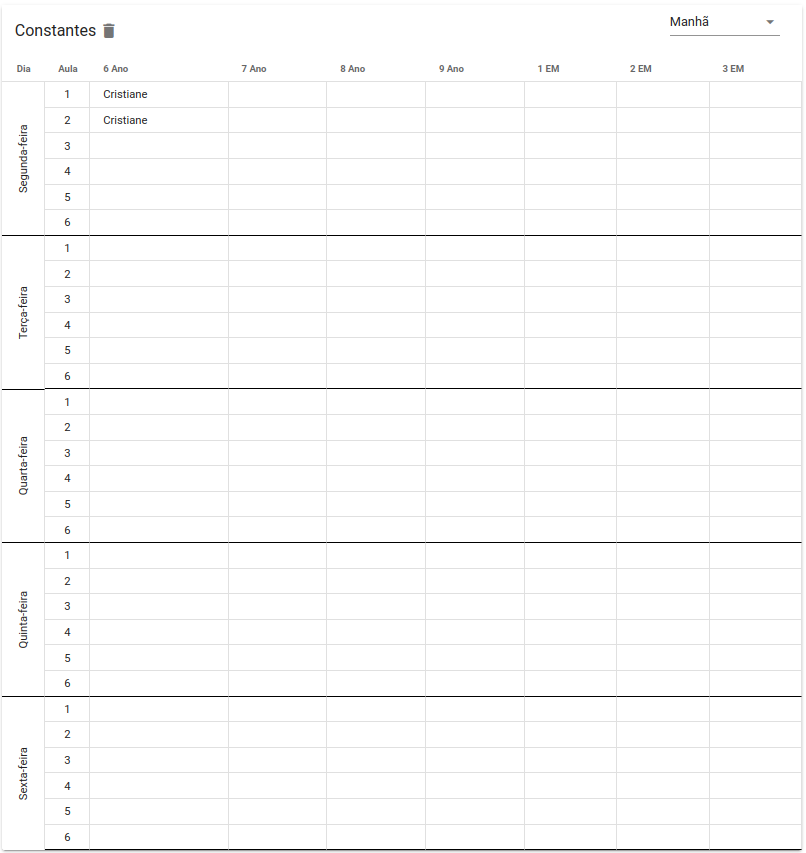
\includegraphics[width=1\textwidth]{./dados/figuras/constantes_configuradas}
	\fonte{Autor}
	\label{fig:constantes_configuradas}
\end{figure}

\begin{figure}[p]
	\centering
	\caption{Restrições e preferências configuradas na interface}
	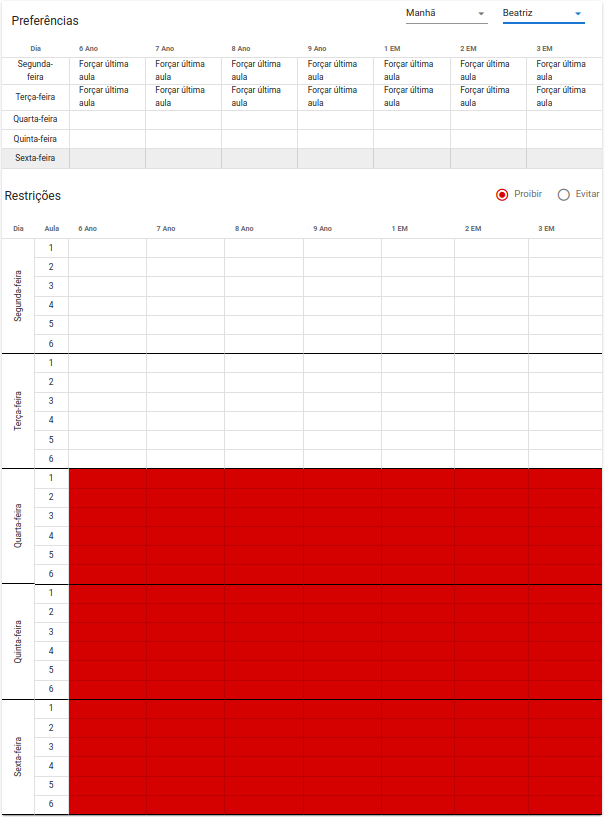
\includegraphics[width=1\textwidth]{./dados/figuras/restricoes_configuradas}
	\fonte{Autor}
	\label{fig:restricoes_configuradas}
\end{figure}

\begin{figure}[p]
	\centering
	\caption{Regiões e grupos de alinhamento configuradas para o turno da ``Manhã''}
	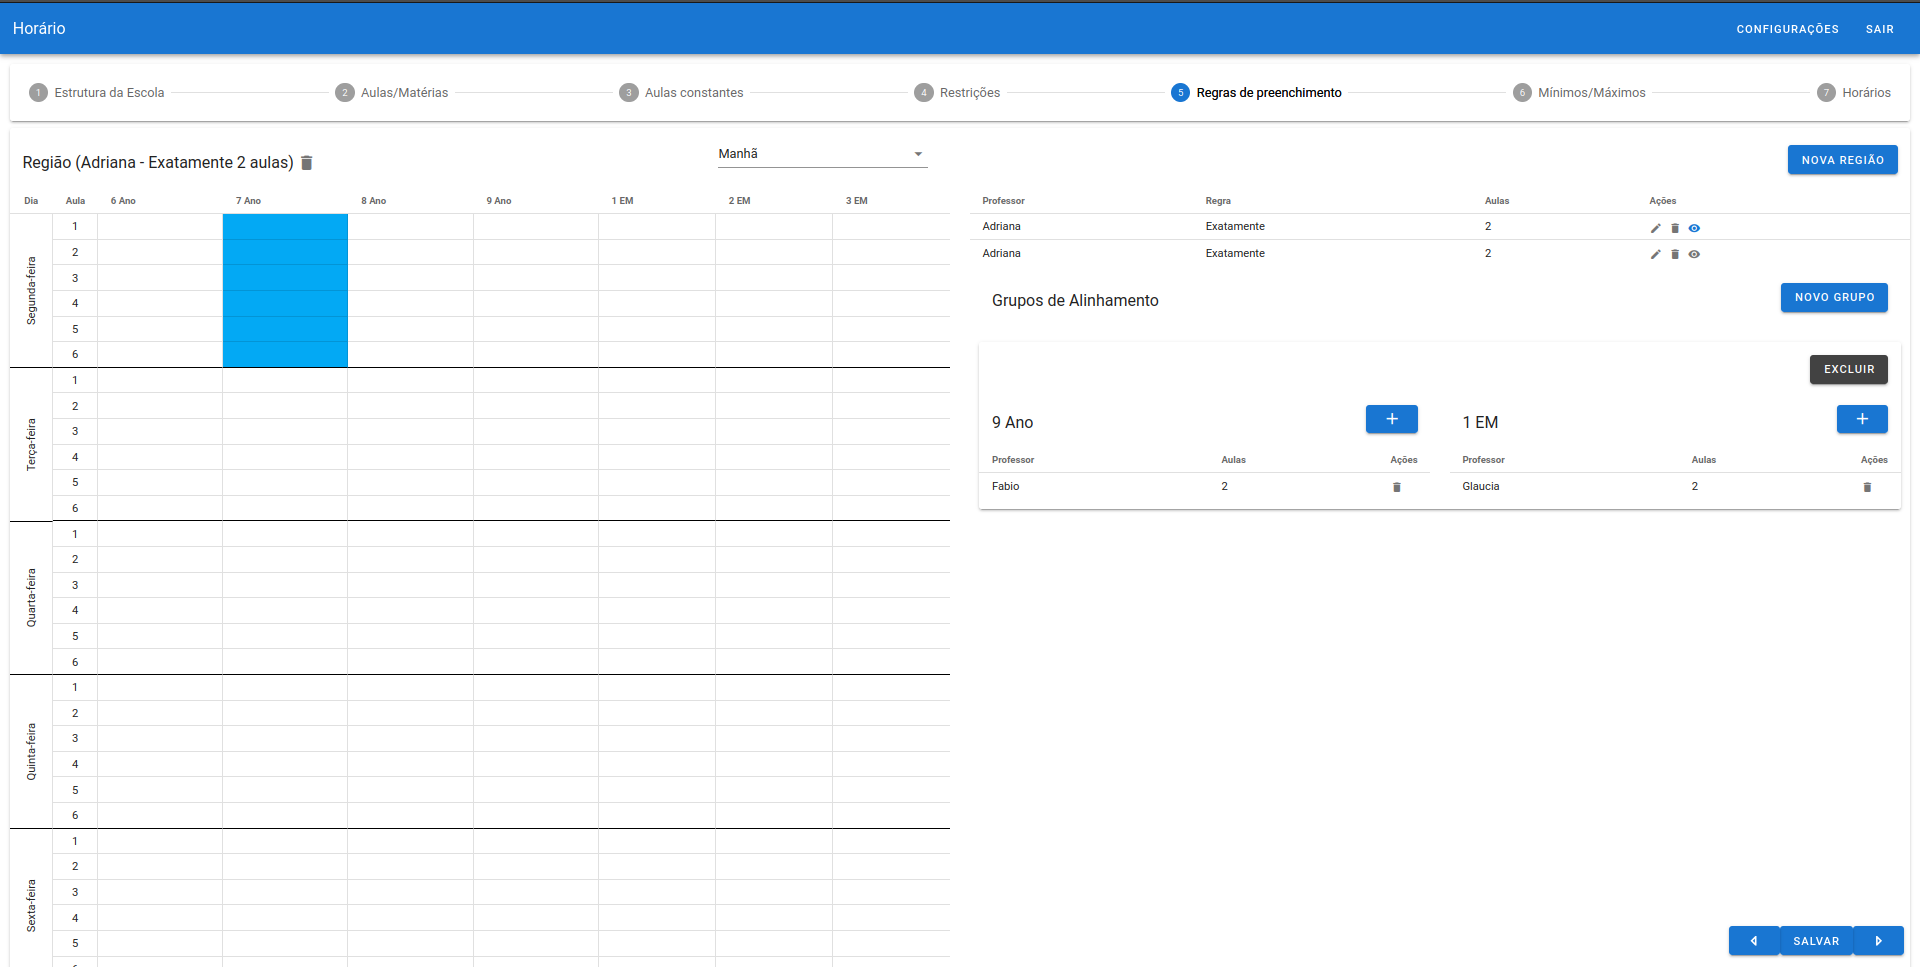
\includegraphics[width=1\textwidth]{./dados/figuras/regioes_configuradas_manha}
	\fonte{Autor}
	\label{fig:regioes_configuradas_manha}
\end{figure}

\begin{figure}[p]
	\centering
	\caption{Regiões e grupos de alinhamento configuradas para o turno da ``Tarde''}
	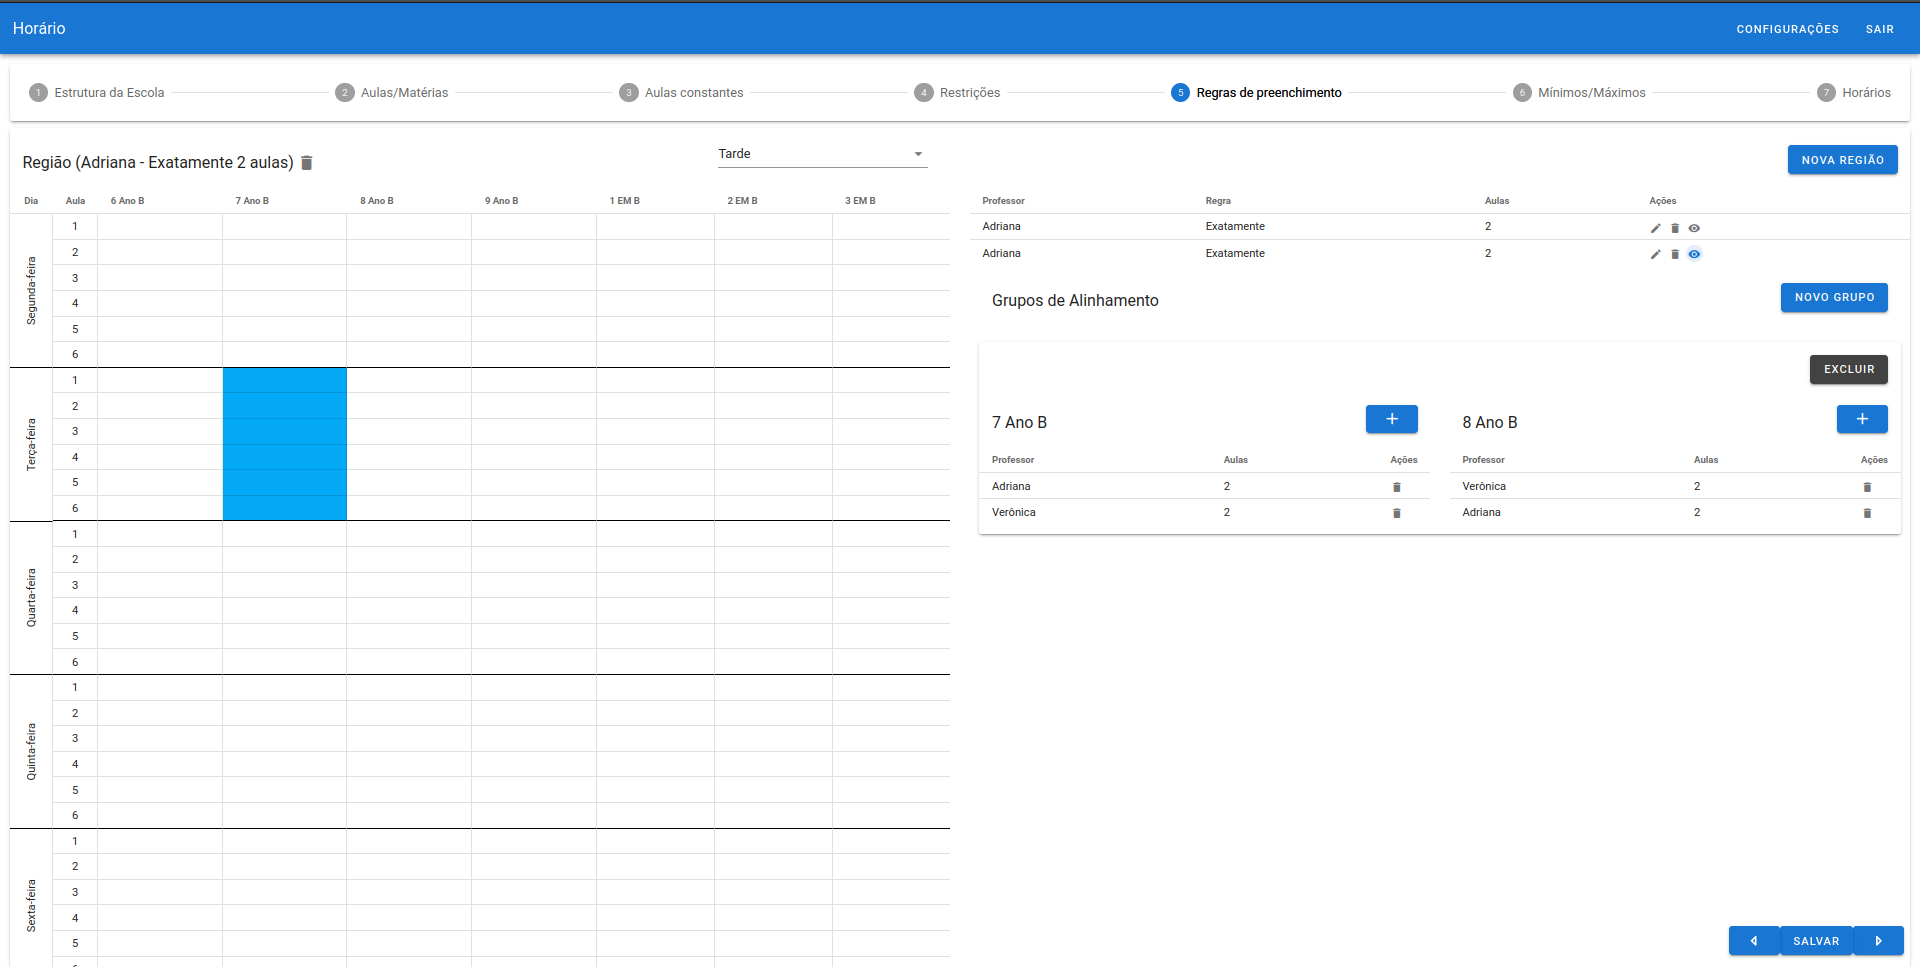
\includegraphics[width=1\textwidth]{./dados/figuras/regioes_configuradas_tarde}
	\fonte{Autor}
	\label{fig:regioes_configuradas_tarde}
\end{figure}

\begin{figure}[h]
	\centering
	\caption{Mínimos de aulas configuradas na interface}
	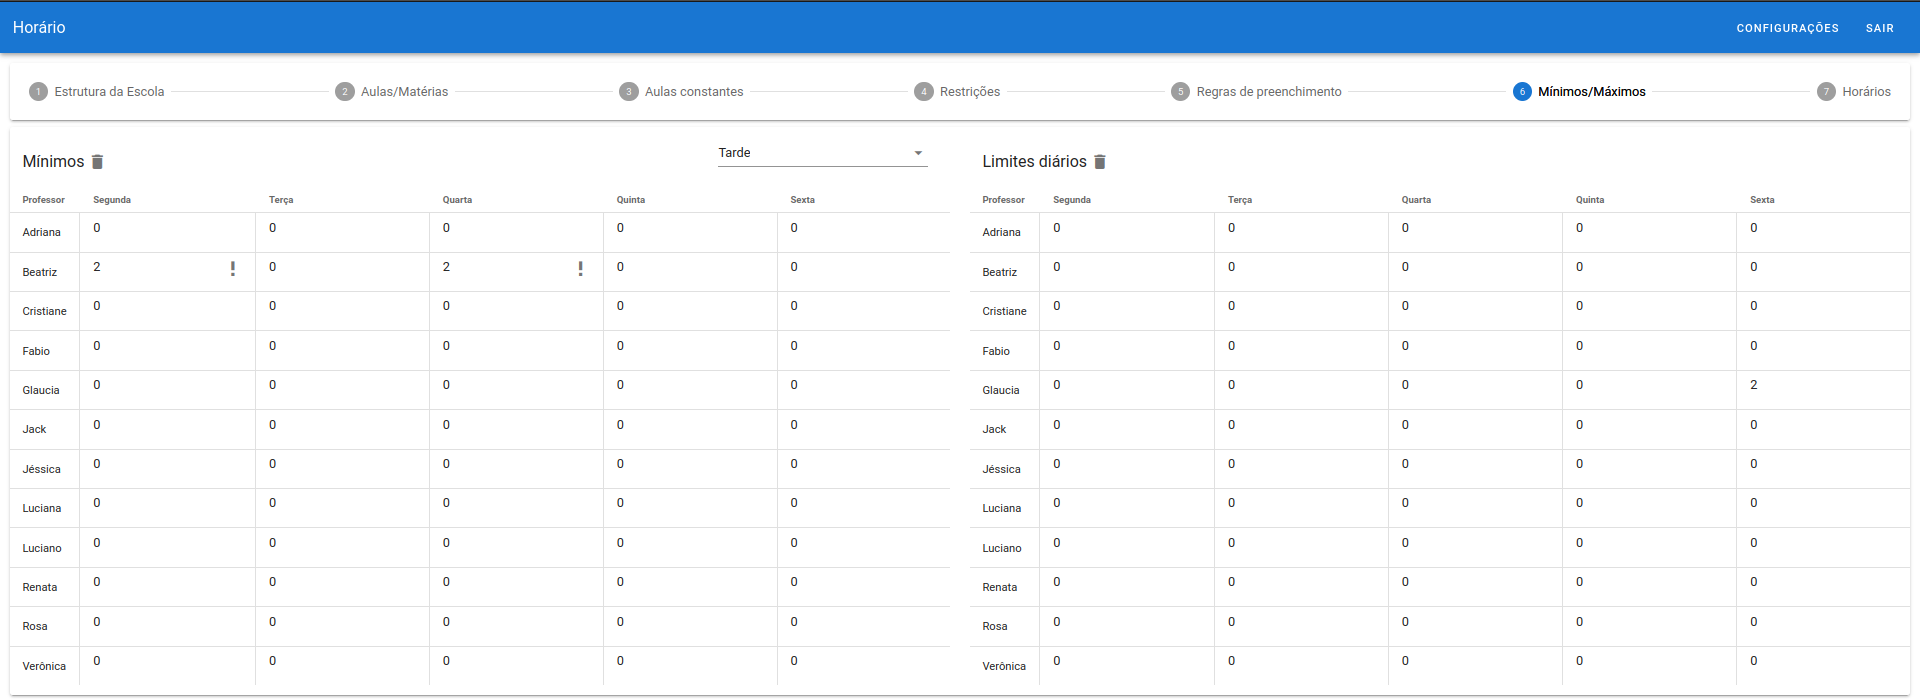
\includegraphics[width=1\textwidth]{./dados/figuras/minimos_configurados}
	\fonte{Autor}
	\label{fig:minimos_configurados}
\end{figure}

\newpage
\begin{enumerate}
	\item \label{item_constantes} \textbf{Constantes}: Conforme a figura \ref{fig:constantes_configuradas}, definiu-se que ``Cristiane'' deveria lecionar as duas primeiras aulas da segunda-feira na turma do ``6º Ano'', em ambos os turnos;
	\item \label{item_restricoes} \textbf{Restrições e preferências}: Na figura \ref{fig:restricoes_configuradas}, é possível notar que no turno da manhã, ``Beatriz'' não deve ter aulas alocadas na quarta, quinta ou sexta-feira. Além disso, informou-se pela interface que suas aulas devem ser lecionadas obrigatoriamente como a última aula do expediente de cada turma;
	\item \label{item_regioes} \textbf{Regiões}: Utilizando o conceito das regiões, definiu-se que ``Adriana'' deveria lecionar exatamente duas aulas para a turma do ``7º Ano'' na segunda-feira, e exatamente 2 aulas para ``7º Ano B'' na terça-feira. Estas configurações abragem tanto o turno da ``Manhã'', quanto da ``Tarde'', como pode ser visto nas figuras \ref{fig:regioes_configuradas_manha} e \ref{fig:regioes_configuradas_tarde};
	\item \label{item_grupos} \textbf{Grupos de alinhamento}: Defniu-se que duas aulas do professor ``Fábio'' no ``9º Ano'' devem ser alocadas simulataneamente a duas aulas da professora ``Glaucia'' no ``1º EM''. Além disso, duas aulas de ``Adriana'' no ``7º Ano B'' devem ser alocadas simulataneamente a duas aulas de ``Verônica'' no ``8º Ano B'', e vice-versa. Assim como as regiões, as configurações dos grupos de alinhamento podem ser conferidas nas figuras \ref{fig:regioes_configuradas_manha} e \ref{fig:regioes_configuradas_tarde};
	\item \label{item_minimos} \textbf{Mínimos e limites diários}: Como pode ser visto na figura \ref{fig:minimos_configurados}, configurou-se que no turno da tarde, ``Beatriz'' deve ministrar no mínimo duas aulas na segunda-feira e 2 aulas na quarta-feira; além disso, ``Gláucia'' deve ministrar no máximo duas aulas na sexta-feira, contabilizando ambos os turnos.
\end{enumerate}

Realizadas as configurações, o otimizador foi ativado, e utilizou-se como condição de parada a passagem de um intervalo de tempo de um minuto. Durante este intervalo, o otimizador produziu 65 soluções plausíveis diferentes, cada qual contendo uma grade horária para o turno da manhã e uma para o turno da tarde.

\begin{figure}[p]
	\centering
	\caption{Visualização de turno da manhã da melhor solução}
	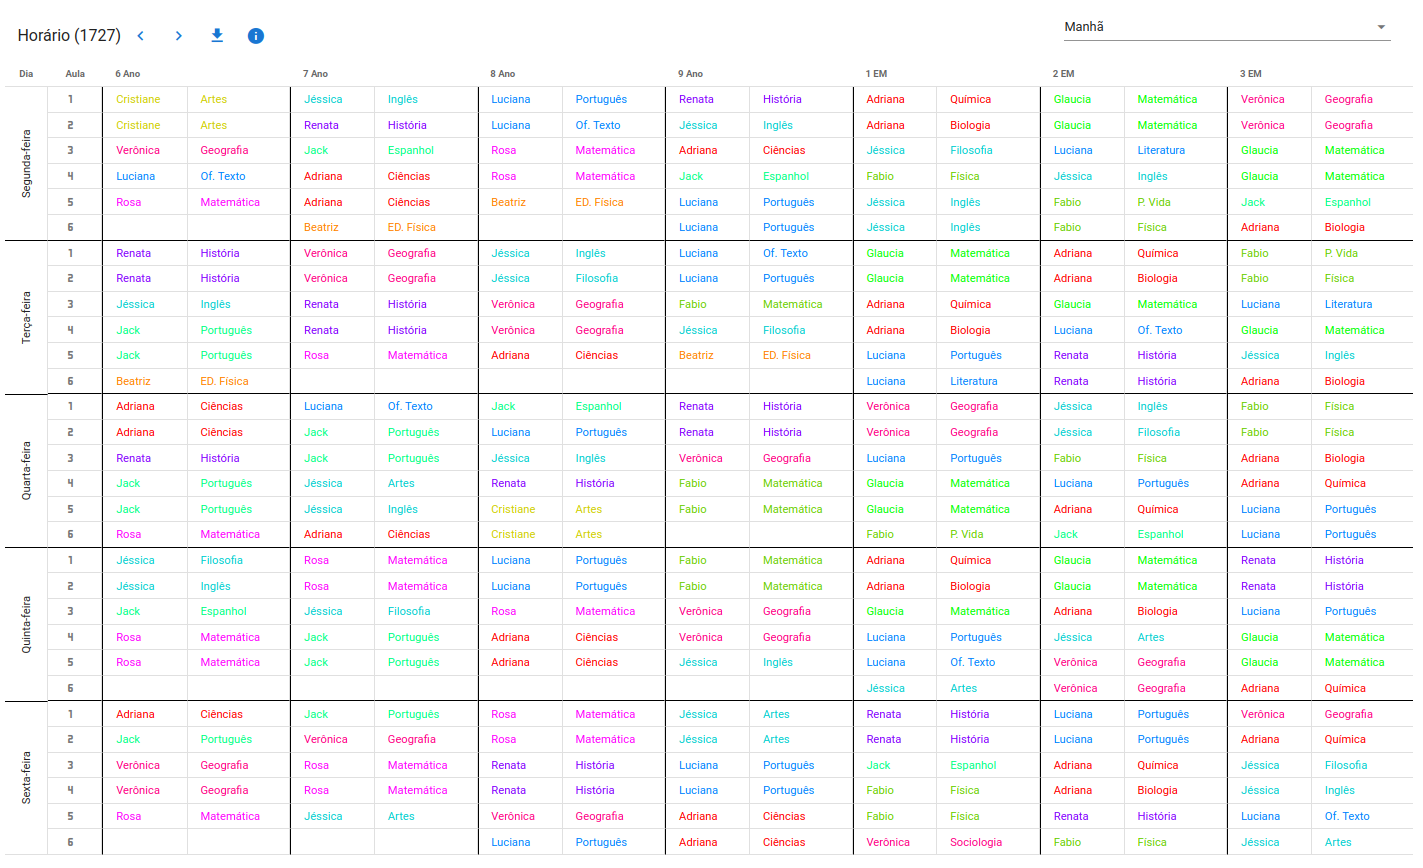
\includegraphics[width=1\textwidth]{./dados/figuras/horario_exportado_manha}
	\fonte{Autor}
	\label{fig:horario_exportado_manha}
\end{figure}

Destas soluções, a melhor encontrada pode ser vista na figura \ref{fig:horario_exportado_manha}, cujas métricas de qualidade foram trasncritas para o quadro \ref{qua:caracteristicas_horario_validacao}. Para melhor leitura e análise, as informações de ambos os turnos da grade gerada foram exportadas para as planilhas nas figuras \ref{fig:planilha_exportada_manha} e \ref{fig:planilha_exportada_tarde}, respectivamente.

\begin{quadro}[p]
	\centering
	\caption{Métricas de qualidade da melhor solução.\label{qua:caracteristicas_horario_validacao}}
	\begin{tabular}{|p{8cm}|p{1cm}|p{3cm}|}
		\hline
		\textbf{Nome} & \textbf{Valor} & \textbf{Tipo} \\
		\hline
		Excessos de matérias iguais & 0 & Rígida \\
		\hline
		Restrições violadas & 0 & Rígida \\
		\hline
		Limites diários violados & 0 & Rígida \\
		\hline
		Aulas em grupos de alinhamento não alinhadas & 0 & Rígida \\
		\hline
		Mínimos opcionais violados & 0 & Rígida \\
		\hline
		Mínimos violados & 0 & Rígida \\
		\hline
		Erros nas regiões & 0 & Rígida \\
		\hline
		Matérias desagrupadas & 0 & Rígida \\
		\hline
		Conflitos & 0 & Rígida \\
		\hline
		Aulas desagrupadas & 0 & Rígida \\
		\hline
		Excessos de aulas iguais & 0 & Rígida \\
		\hline
		Dias com todos professores diferentes & 0 & Rígida \\
		\hline
		Restrições opcionais violadas & 0 & Suave \\
		\hline
		Horários com janela (total de todos professores) & 1 & Suave \\
		\hline
		Número de grupos de alinhamento formados & 4 & Suave \\
		\hline
		Preferências não resolvidas & 0 & Suave \\
		\hline
		Aulas separadas & 142 & Suave \\
		\hline
		Dias de professores sem aulas duplas & 0 & Suave \\
		\hline
		Matérias separadas & 208 & Suave \\
		\hline
	\end{tabular}
	\fonte{Autoria própria}
\end{quadro}

\begin{figure}[p]
	\centering
	\caption{Grade exportada - Turno da Manhã}
	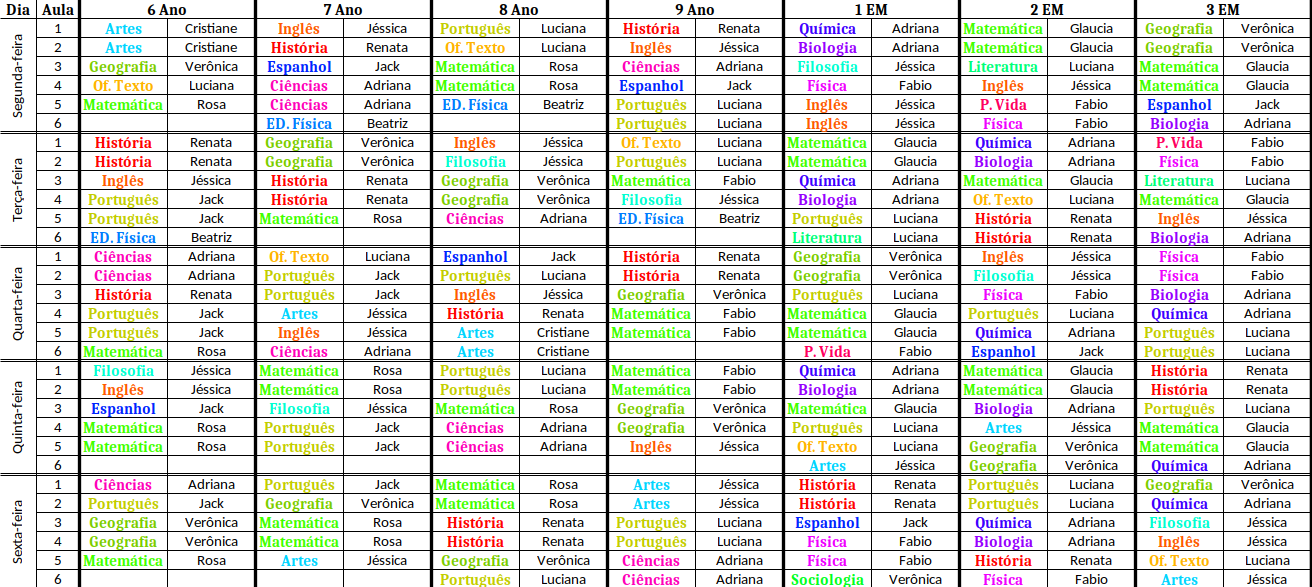
\includegraphics[width=1\textwidth]{./dados/figuras/planilha_exportada_manha}
	\fonte{Autor}
	\label{fig:planilha_exportada_manha}
\end{figure}

\begin{figure}[p]
	\centering
	\caption{Grade exportada - Turno da Tarde}
	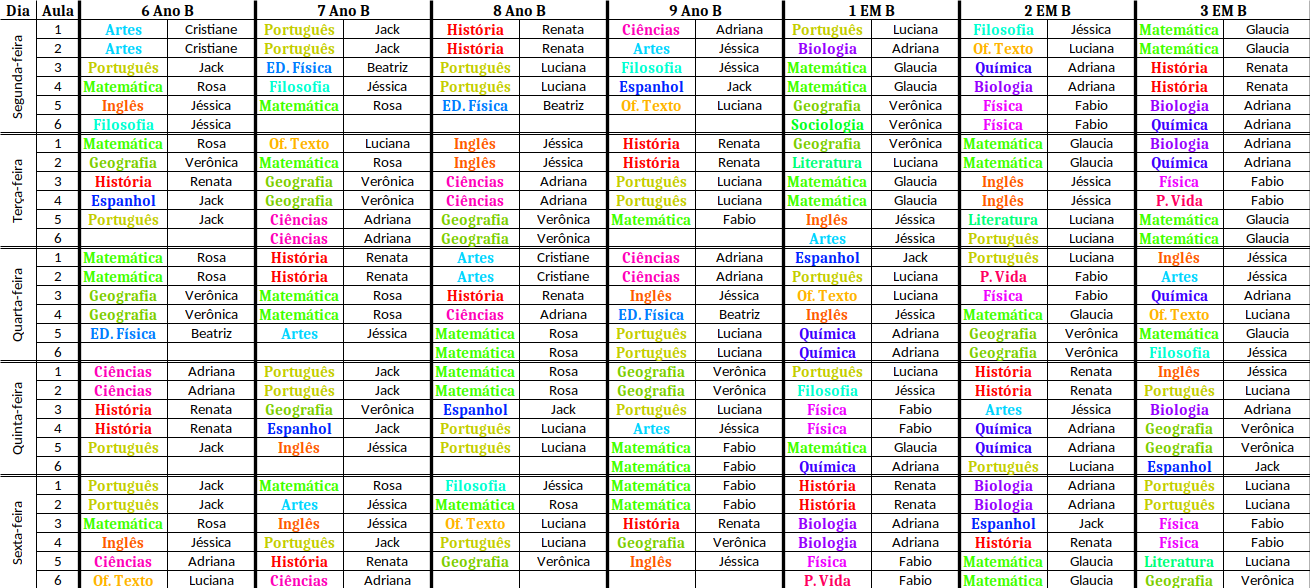
\includegraphics[width=1\textwidth]{./dados/figuras/planilha_exportada_tarde}
	\fonte{Autor}
	\label{fig:planilha_exportada_tarde}
\end{figure}

\newpage
Observando as figuras \ref{fig:planilha_exportada_manha} e \ref{fig:planilha_exportada_tarde}, constata-se que:

\begin{enumerate}
	\item Foi alocada a quantidade correta de aulas para cada professor e matéria, nas salas corretas, de acordo com o quadro \ref{qua:validacao};
	\item As aulas foram alocadas sem causar conflitos, ou seja, em nenhum horário das grades, um professor está alocado para mais de uma turma simultaneamente;
	\item Aproximadamente 64\% das aulas foram agrupadas: conforme o quadro \ref{qua:caracteristicas_horario_validacao}, apenas 142 do total de 396 aulas permaneceram separadas;
	\item As aulas constantes mencionadas no item \ref{item_constantes} foram alocadas corretamente: Cristiane foi alocada nas duas primeiras aulas da segunda-feira na turma do 6º Ano e 6º Ano B;
	\item As restrições e preferências do item \ref{item_restricoes} foram atendidas: ``Beatriz'' não teve aulas alocadas na quarta, quinta ou sexta-feira no turno da manhã, e neste mesmo turno suas aulas ocuparam sempre os últimos horários do expediente de cada turma;
	\item Em conformidade com o item \ref{item_regioes}, na segunda-feira a professora ``Adriana'' teve exatamente duas aulas alocadas na turma do ``7º Ano'', e duas no ``7º Ano B'';
	\item O grupo de alinhamento da figura \ref{fig:regioes_configuradas_manha} foi respeitado, já que duas aulas do professor ``Fábio'' no ``9º Ano'' foram alocadas simultaneamente a duas aulas de ``Adriana'' no ``1º EM''. As aulas do grupo da figura \ref{fig:regioes_configuradas_tarde} também foram alocadas corretamente;
	\item As quantidades mínimas e máximas de aulas do item \ref{item_minimos} foram respeitadas: foram alocadas para ``Beatriz'' exatamente duas aulas na segunda e quarta-feira no período da tarde; e exatamente duas aulas para ``Gláucia'' na sexta-feira, somando as aulas de ambos os turnos;
\end{enumerate}      


